%\documentclass[preprint,tightenlines,showpacs,showkeys,floatfix,
%nofootinbib,superscriptaddress,fleqn]{revtex4} 
\documentclass[floatfix,nofootinbib,superscriptaddress,fleqn,preprint]{revtex4} 
%\documentclass[aps,epsfig,tightlines,fleqn]{revtex4}
\usepackage[utf]{kotex}
\usepackage[HWP]{dhucs-interword}
\usepackage[dvips]{color}
\usepackage{graphicx}
\usepackage{bm}
%\usepackage{fancyhdr}
%\usepackage{dcolumn}
\usepackage{defcolor}
\usepackage{amsmath}
\usepackage{amsfonts}
\usepackage{amssymb}
\usepackage{amscd}
\usepackage{amsthm}
\usepackage[utf8]{inputenc}
 \usepackage{setspace}
%\pagestyle{fancy}

\begin{document}

\title{\Large 2022년 1학기 물리학 I: Quiz 4}
\author{김현철\footnote{Office: 5S-436D (면담시간 매주
    화요일-16:00$\sim$20:00)}} 
\email{hchkim@inha.ac.kr}
\author{Lee Hui Jae} 
\email{hjlee6674@inha.edu}
\affiliation{Hadron Theory Group, Department of Physics, Inha University,
Incheon 402-751, Republic of Korea }
\date{Spring semester, 2022}


\vspace{1.cm}
\begin{abstract}
\noindent \textbf{ {\color{red}주의}: \color{blue} 단 한 번의 부정행위도 절대
  용납하지 않습니다. 적발 시, 학점은 F를 받게 됨은 물론이고,
  징계위원회에 회부합니다. One strike out임을 명심하세요.}\\
\\
문제는 다음 쪽부터 나옵니다.  \\ \\
{\bf Date:} 2022년 3월 14일 (월) 15:30--16:15
\\
{\bf 학번:} \hspace{4cm}
{\bf 이름:} 

\end{abstract}
\maketitle

\noindent {\bf 문제 1 [10pt]} 
그림~\ref{fig:1}과 같이 어떤 사람이 건물
꼭대기에서 수평에서부터 $30^\circ$의 각도로, 20.0 m/s의 속도로
공을 던졌다. 건물 
바닥에서 공을 던진 곳까지 높이는 45.0 m이다. 
\begin{figure}[ht]
  \centering
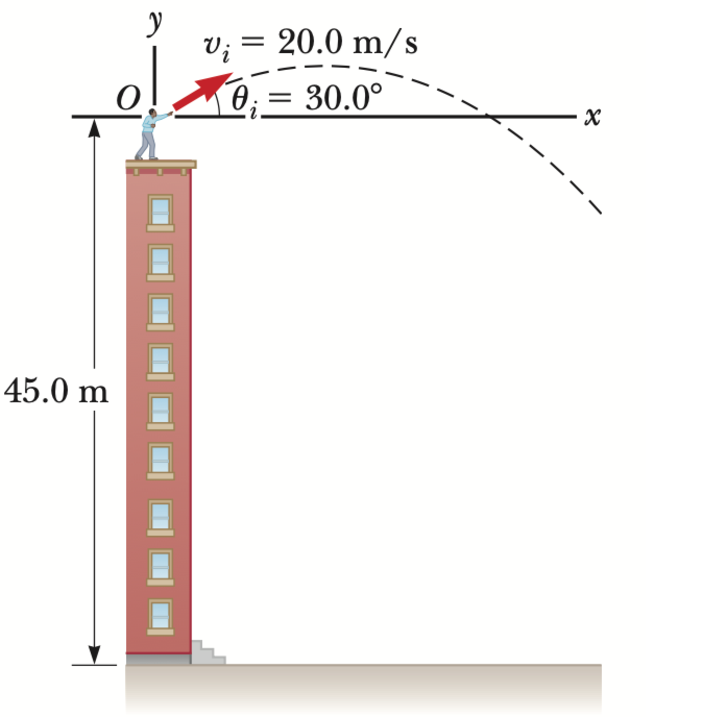
\includegraphics[scale=0.6]{Qfig4-2.pdf}  
  \caption{문제 2}
  \label{fig:1}
\end{figure}
\begin{itemize}
\item[(가)] 공이 지면에 닿을 때까지 걸린 시간을 구하여라.
\item[(나)] 공이 지면에 닿을 때 속력을 구하여라. (이 문제에서는 계산기를
  쓰셔도 무방합니다.)
\end{itemize}
\noindent {\bf 해답}
\begin{itemize}
  \item[(가)]공은 중력에 의한 포물선 운동을 하므로, 수직 방향 운동과
  수평 방향 운동을 따로 생각할 수 있다. 수직 방향으로는 중력에 의한 등가속도 운동을 하게 된다.
  이 공의 초기 수직 방향 속력은 다음과 같다.
  \begin{align}
    v_{x,0}=v_i\sin{\theta_i}=(20.0\,\mathrm{m/s})\sin{30^\circ}
    =(20.0\,\mathrm{m/s})\left(\frac{1}{2}\right)
  \end{align}
  중력은 아래 방향으로 작용하므로,
  시간 $t$ 일 때 이 공의 위치는 다음과 같다.
  \begin{align}
    x=x_0+v_0t-\frac{1}{2}gt^2
  \end{align}
  $v_0=v_{x,0}$ 이고, 초기 위치는 45 m, 나중 위치는 0 m 이므로,
  \begin{align}
    \begin{split} 
      0\,\mathrm{m}&=45\,\mathrm{m}+(20.0\,\mathrm{m/s})
      \left(\frac{1}{2}\right)\times t
      -\left(\frac{1}{2}\right)
      (9.80\,\mathrm{m/s^2})\times t^2 \\
      &=45\,\mathrm{m}+(10.0\,\mathrm{m/s})\times t
      -(4.90\,\mathrm{m/s^2})\times t^2.
    \end{split}
  \end{align}
  이는 $t$ 에 대한 2차 방정식이다. 해는 $t=-2.18\,\mathrm{s} $ 
  그리고 $t=4.22\,\mathrm{s}$ 이다. 
  따라서, 걸린 시간은 $4.22\,\mathrm{s}$ 이다.
  \item[(나)] 
  수평 방향으로는 가속도가 존재하지 않기 때문에 수평 방향 속력은 
  변하지 않는다. 수평 방향 속력은 다음과 같다.
  \begin{align}
    v_y=v_i\cos{\theta_i}=(20.0\,\mathrm{m/s})\cos{30^\circ}
    =(20.0\,\mathrm{m/s})\left(\frac{\sqrt{3}}{2}\right)
  \end{align}
  수직 방향 속력은 중력 가속도를 받아 지면에 닿을 때 까지 일정하게 변한다. 
  지면에 닿을 때 수직 방향 속력은 다음과 같다.
  \begin{align}
    v_x=v_{x,0}-gt=v_i\sin{\theta_i}-gt
    =(20.0\,\mathrm{m/s})\left(\frac{1}{2}\right)
    -(9.80\,\mathrm{m/s^2})(4.22\,\mathrm{s})
  \end{align}
  이 공의 전체 속력은 다음과 같다.
  \begin{align}
    \begin{split}
      v&=\sqrt{v_x^2+v_y^2}=\sqrt{{(v_i\sin{\theta_i}-gt)}^2+{(v_i\cos{\theta_i})}^2} \\
      &=\sqrt{{\left((20.0\,\mathrm{m/s})\left(\frac{1}{2}\right)
      -(9.80\,\mathrm{m/s^2})(4.22\,\mathrm{s})\right)}^2
      +{\left((20.0\,\mathrm{m/s})\left(\frac{\sqrt{3}}{2}\right)\right)}^2}  \\
      &=\sqrt{{\left((10.0\,\mathrm{m/s})
      -(41.4\,\mathrm{m/s})\right)}^2
      +{\left((10.0\,\sqrt{3}\,\mathrm{m/s})\right)}^2} \\
      &=\sqrt{986+300}\,\mathrm{m/s}\\
      &=35.86\,\mathrm{m/s}
    \end{split}
  \end{align}
  공이 지면에 닿을 때 속력은 $35.86\,\mathrm{m/s}$ 이다.
\end{itemize}

\vspace{2cm}

\noindent {\bf 문제 2 [20pt]} 초기 위치 $x_0$, 초기 속력 $v_0$이
주어졌을 때, 아래의 식
\begin{align}
  \label{eq:1}
v^2 - v_0^2 = 2a(x-x_0)  
\end{align}
을 다음과 같이 유도해보자. 순간 가속도는
\begin{align}
  \label{eq:2}
a = \frac{dv}{dt}
\end{align}
와 같이 주어진다. \eqref{eq:2}의 양변에 속력 $v$를 곱한 식에서부터
\eqref{eq:1}을 유도하여라. (적분을 이용하여야 한다는 점을 명심하여라.)  \\
\noindent {\bf 해답} \eqref{eq:2}의 양변에 속력 $v$를 곱하면,
\begin{align}
  a\,v(t) = v(t)\frac{dv}{dt}.
\end{align}
양변을 $t^\prime$ 에 대해 $t^{\prime}=t_0$ 부터 $t^\prime=t$ 까지 적분하자.
\begin{align}\label{eq:3}
  \begin{split}
    \int_{t_0}^t a\,v(t^\prime)\,dt^\prime 
    &=\int_{t_0}^t v(t^\prime)\frac{dv}{dt^\prime}\,dt^\prime  \\
    &= \int_{v_0}^v v(t^\prime)\,dv(t^\prime)
    =\frac{1}{2}\left(v^2-v^2_0\right)
  \end{split}
\end{align} 
속력은 위치를 시간에 대해 미분한 값이다. 따라서,
\begin{align}
  v(t)=\frac{dx(t)}{dt}.
\end{align}
\eqref{eq:3}의 좌항에 대입하고 부분적분 하자.
\begin{align}
  \int_{t_0}^ta\,\frac{dx}{dt^\prime}\,dt^\prime
  =a\,x(t^\prime)|_{0}^t-\int_{t_0}^t\frac{da}{dt^\prime}\,x(t^\prime) \,dt^\prime
\end{align}
등가속도 운동에서는 가속도가 일정하므로 다음과 같다.
\begin{align}
  a\,x(t^\prime)|_{0}^t-\int_{t_0}^t\frac{da}{dt^\prime}\,x(t^\prime) \,dt^\prime
  =a\left(x-x_0\right)-\int_{t_0}^t0\,x(t^\prime) \,dt^\prime
  =\frac{1}{2}\left(v^2-v^2_0\right)
\end{align}
최종적으로,
\begin{align}
  v^2 - v_0^2 = 2a(x-x_0).
\end{align}
%\begin{align}
%  \int_{t_0}^t av\,dt = \int_{t_0}^t v\frac{dv}{dt}\,dt 
%  = \left[ 2v \right]_{t_0}^t = 2(v-v_0).
%\end{align}

\vspace{2cm}

\noindent {\bf 문제 3 [10pt]} 
스키 점프 선수가 트랙의 수평면에 도달해서
수평방향으로 도약을 했다. 이 때 속력은 25.0 m/s였다. 그리고 수평면과
경사면 사이의 각은 $35.0^\circ$였다. 이 선수는 어느 지점에 착지했을까? 
\begin{figure}[ht]
  \centering
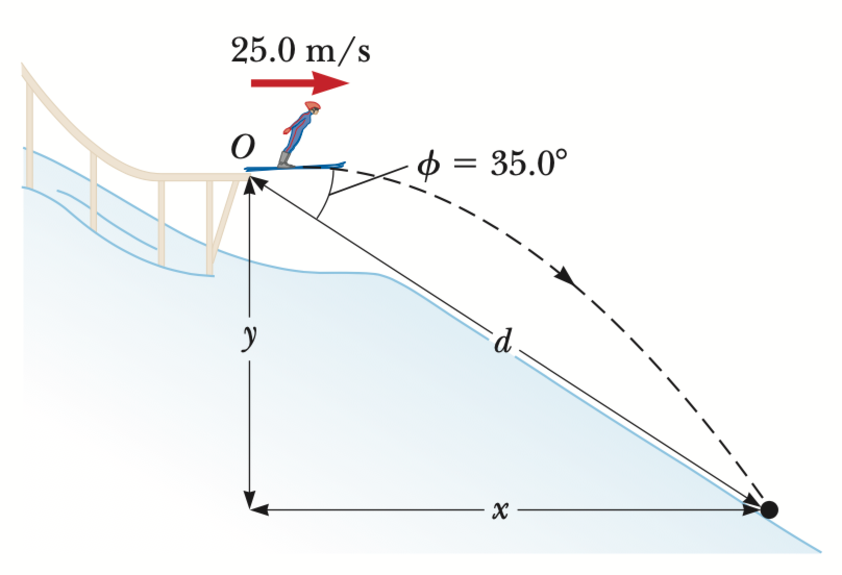
\includegraphics[scale=0.6]{Qfig4-3.pdf}  
  \caption{문제 3}
  \label{fig:2}
\end{figure}

\noindent {\bf 해답} 스키 점프 선수가 도약한 지점으로 부터 착지한 지점까지 
수평 방향으로 떨어진 거리를 $x$, 수직 방향으로 떨어진 거리를 $y$ 라 하자.
$x$ 와 $y$ 의 관계는 삼각비로 표현할 수 있다.
\begin{align}\label{eq:4}
  \frac{y}{x}=\tan{\phi}
\end{align}
스키 점프 선수가 도약하는 동안 수평 방향으로 이동한 거리 $x$ 는 다음과 같다.
\begin{align}
  x=v_xt=(25.0\,\mathrm{m/s})t 
\end{align}
수직 방향으로는 중력 가속도가 존재하여 등가속도 운동한다. 따라서, 수직 방향으로
이동한 거리 $y$ 는 다음과 같다.
\begin{align}
  y=v_{y,0}t+\frac{1}{2}gt^2=\frac{1}{2}gt^2=\frac{1}{2}(9.80\,\mathrm{m/s^2})t^2
\end{align}
관계식 (\ref{eq:4}) 에 대입하면 다음과 같다.
\begin{align}
  \tan{\phi} = \frac{y}{x} = \frac{\frac{1}{2}gt^2}{v_xt}=\frac{gt}{2v_x},\,\,\,
  t=\frac{2v_x\tan{\phi}}{g}
\end{align}
도약한 지점과 착지한 지점 사이 거리를 $d$ 라 하면, 
\begin{align}
  \begin{split}
    d&=\sqrt{x^2+y^2}=x\sqrt{1+\left(\frac{y}{x}\right)^2}=v_xt\sqrt{1+\tan^2{\phi}} \\
    &=\frac{2v_x^2\tan{\phi}}{g}\sqrt{1+\tan^2{\phi}}
  \end{split}
\end{align}
이다.
경사면의 각도는 $35.0^\circ$ 이고 수평 방향 속력은 $25.0\,\mathrm{m/s}$ 이므로 $d$ 는
다음과 같다.
\begin{align}
  \begin{split}
    d&=\frac{2(25.0\,\mathrm{m/s})^2\tan{35.0^\circ}}{(9.80\,\mathrm{m/s^2})}\sqrt{1+\tan^2{35.0^\circ}} \\
    &= \frac{2(25.0\,\mathrm{m/s})^2 (0.700)}{(9.80\,\mathrm{m/s^2})}\sqrt{1+(0.700)^2} \\
    &= (89.3\,\mathrm{m})(1.22) = 109\,\mathrm{m} \\
  \end{split}
\end{align}
스키 점프 선수는 도약 지점으로 부터 109 m 떨어진 지점에 착지했다.
%\begin{align}
%\tan{\phi}=\tan{35.0^\circ}=\frac{y}{x}
%=\frac{(9.80\,\mathrm{m/s^2})t^2}{2(25.0\,\mathrm{m/s})t }=
%\end{align}

\vspace{2cm}


\noindent {\bf 문제 4 [10pt]} 높이가 $y_0=15.0$ m인 건물이 있다. 이 건물
꼭대기에서 $v_0=10.0$ m/s의 속력으로 위로 공을 쏘아올렸다. 
\begin{figure}[ht]
  \centering
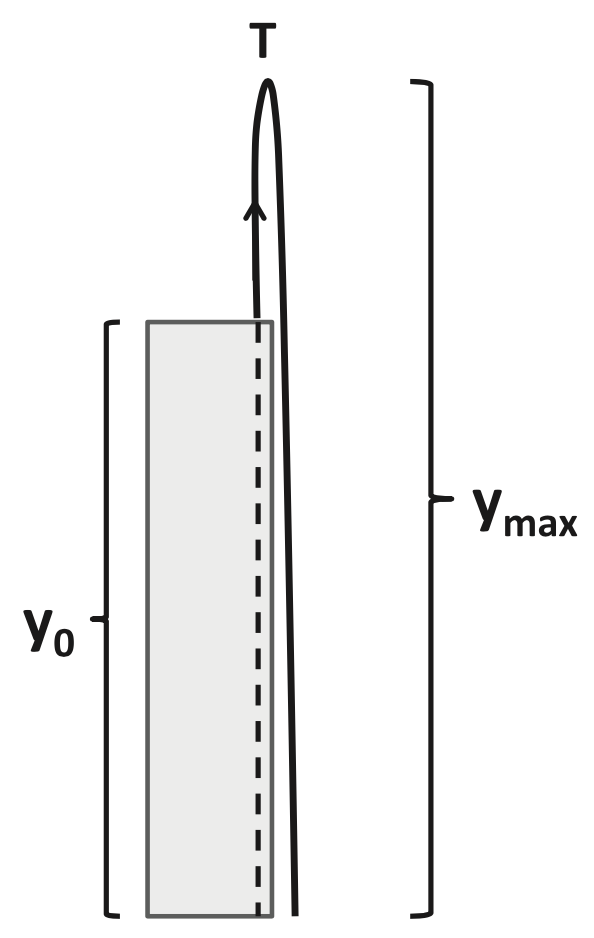
\includegraphics[scale=0.5]{Qfig4-4-20210312.png}  
  \caption{문제 4}
  \label{fig:4}
\end{figure}
그림~\ref{fig:4}에 보여주는 $y_{\mathrm{max}}$를 구하여라. 

\noindent {\bf 해답} 이 공은 중력에 의한 등가속도 운동을 
하고 있으므로 공의 높이는 다음과 같다.
\begin{align}
  y=y_0+v_0t-\frac{1}{2}gt^2
\end{align}
$t$ 에 대한 완전제곱 꼴로 바꾸면,
\begin{align}
  y=-\frac{1}{2}g\left( t-\frac{v_0}{g} \right)^2+\frac{v_0^2}{2g}+y_0
\end{align}
$y$ 의 최댓값이 다음과 같음을 볼 수 있다.
\begin{align}
  y_{\mathrm{max}}=\frac{v_0^2}{2g}+y_0
\end{align}
초기 높이가 15.0 m, 초기 속력은 10.0 m/s 이므로, $y_{\mathrm{max}}$ 는 다음과 같다.
\begin{align}
  \begin{split}
    y_{\mathrm{max}}&=\frac{v_0^2}{2g}+y_0 
    = \frac{(10.0\,\mathrm{m/s})^2}{2(9.80\,\mathrm{m/s^2})}+15.0\,\mathrm{m} \\
    &=5.10\,\mathrm{m}+15.0\,\mathrm{m} \\
    &=20.1\,\mathrm{m}
  \end{split}
\end{align}
이 공은 지면으로부터 최대 20.1 m 까지 올라간다.
\end{document}